\documentclass{article}[12pt]

\usepackage{graphicx}
\usepackage{subfig}
\usepackage[margin=1in]{geometry}
\usepackage{algorithm}
\usepackage[noend]{algpseudocode}
\usepackage{amsmath}
\usepackage[font=small,skip=0pt]{caption}

\begin{document}
	\begin{titlepage}
		\centering
		{\scshape\huge MASTER DEGREE OF RESEARCH IN ARTIFICIAL INTELLIGENCE \par}
		\vspace{1cm}
		{\scshape\large Course 2019-2020 \par}
		\vspace{1cm}
		{\scshape\huge \bf{Assignment 3.6: Comparison of a population-based algorithm and a trajectory algorithm} \par}
		\vspace{1cm}
		{\scshape\LARGE \it{Luis Gonzalez Naharro} \par}
		\vspace{1cm}
		{\scshape\large \today \par}
		\vspace{1cm}
		{\scshape\large \line(1,0){250} \par}
		\vspace{.2cm}
		
\includegraphics[width=.8\linewidth]{../UIMP}
		
\includegraphics[width=.8\linewidth]{../AEPIA}
	\end{titlepage}
	
	\tableofcontents
	
	\newpage
	
	\listoffigures
	
	\newpage
	
	\listofalgorithms
	
	\newpage
	
	\listoftables
	
	\newpage
	
	\section{Introduction}
	The objective of this work is to perform a comparison between a couple of metaheuristic algorithms: a population-based algorithm (namely, a genetic algorithm) and a trajectory-based algorithm (namely, a simulated annealing algorithm), in order to determine which one behaves better under a set of pre-established conditions.
\bigbreak
	As it is known, there is a class of computational problems known as NP (\textbf{Non-deterministic Polynomial}) problems, which cannot be solved on a feasible amount of time due to their computational complexity increasing exponentially as the size of the input increases. In order to tackle these problems in a more computationally cheap way, a special kind of algorithms named \textbf{metaheuristic algorithms} were developed, which can give approximate optimal solutions to these problems with a minimal amount of problem-specific-tailoring work. However, these algorithms do not guarantee to give the best solution (global optimum). Instead, they almost always give slightly worse solutions (local optima) which, in practice, tend to be very good. This fact, combined with their relatively cheap behavior, has led to their application in many fields, such as logistics, smart cities, etc.
\bigbreak
	The rest of this report is organized as follows: Section \ref{Implementation} details the implementation of the code for running the experiments, Section \ref{Experiments} details the experiments that have been carried out, Section \ref{Results} shows the results of the experiments and analyses them. Finally, Section \ref{Conclusions} gives conclusions about the work done.
	
	\section{Technical implementation} \label{Implementation}
	
	The first task carried out in this work has been implementing the code needed for running the experiments. More specifically, code was needed for the following algorithms:
	
	\begin{itemize}
		\item \textbf{Genetic Algorithm}: this algorithm simulates the behavior of evolution in nature. To do so, it starts from an initial population that evolves by applying selection, crossover and mutation operands during a series of timesteps. This can be seen in more detail on Algorithm \ref{genetic}. Usually, the operators are defined as it follows:
		\begin{itemize}
			\item \textit{Selection}: the best solutions from the population are selected. There are various strategies for this process, such as Roulette Wheel Selection, Tournament Selection, etc.
			\item \textit{Crossover}: the previously chosen solutions are combined two-by-two to generate new solutions with characteristics from both their ``parent'' solutions. The crossover technique is heavily dependant on the problem and the solution codification.
			\item \textit{Mutation}: the resulting ``children'' are mutated by randomly altering elements from their solution. Once again, this process depends on the problem and the codification of the solution.
		\end{itemize}
		
		\item \textbf{Simulated Annealing}: this algorithm simulates the annealing process in metallurgy, by allowing the current solution to change with a high probability to a worse solution in the beginning, and gradually decreasing this probability over time. This can be seen in more detail on Algorithm \ref{annealing}.
	\end{itemize}
	
	\begin{algorithm}
	\caption{Genetic algorithm}\label{genetic}
	\begin{algorithmic}[1]
		\Procedure{geneticAlgorithm}{population}
			\State $t := 0$
			\State $\texttt{initialize}(population)$
			\State $\texttt{evaluate}(population)$
			\While {$\texttt{not stopCondition}()$}
				\State $newPopulation := \texttt{selection}(population)$
				\State $newPopulation \gets \texttt{crossover}(newPopulation)$
				\State $newPopulation \gets \texttt{mutation}(newPopulation)$
				\State $\texttt{evaluate}(newPopulation)$
				\State $population \gets \texttt{replace}(population, newPopulation)$
				\State $t \gets t + 1$
			\EndWhile
			\Return $\texttt{bestSolution}(population)$
		\EndProcedure
	\end{algorithmic}
	\end{algorithm}
	
	\begin{algorithm}
	\caption{Simulated annealing}\label{annealing}
	\begin{algorithmic}[1]
		\Procedure{SimulatedAnnealing}{temperature, coolingRate}
			\State $solution := \texttt{initialize}()$
			\While {$\texttt{not stopCondition}()$}
				\State $newSolution := \texttt{randomNeighbour}(solution)$
				\If {$\texttt{acceptProbability}(solution, newSolution, temperature) > \texttt{random}(0,1)$}
					\State $solution \gets newSolution$
				\EndIf
				 \State $temperature \gets \texttt{decreaseTemperature}(temperature, coolingRate)$
			\EndWhile
			\Return $solution$
		\EndProcedure
	\end{algorithmic}
	\end{algorithm}
	
	While the genetic algorithm was already implemented in the given code at \cite{codigoga}, the implementation of the simulated annealing had to be done manually, by working over the already existing code. Another part that had to be implemented was the knapsack problem; more specifically, the \textbf{m-dimensional knapsack problem}, as stated in the given font at \cite{knapsack}. This problem is very similar to the original knapsack problem, with the difference that each item not only has weight but also a certain number of other unrelated constraints. The knapsack also has limit values for these constraints, and all of them must be met in order to have a valid solution.
\bigbreak
	Another issue that had to be fixed in the base program was the random seeds. The way it was before any modifications, the random values were purely random, without setting any seeds, thus leading to different behavior between executions and impeding the execution of certain statistical tests. The program has been modified so as to be able to set a certain seed in the command line, and to guarantee result reproducibility. In addition, the program has also been modified to set the parameters of each metaheuristic algorithm also in the command line, in order to make an automated script to collect all the required metrics.
	
	\section{Experiments} \label{Experiments}
	
	As it is stated in the description of the assignment, the experiments must be carried out by tuning the hyperparameters of both the Genetic Algorithm and the Simulated Annealing. The parameters of the Genetic Algorithm already work well enough as they are on the code, so they have not been modified. However, the parameters for Simulated Annealing had to be manually tuned. While setting the cooling rate has been done on a trial-and-error basis, the starting temperature has been tuned with the method explained in \cite{saparam}.
\bigbreak
	Two kinds of experiments have been run, as it is asked on the description of the assignment:
	\begin{itemize}
		\item Leaving a very limited number of iterations (\textbf{500000} for these experiments), and returning the best fitness value obtained by the program.
		\item Leaving a high number of iterations (\textbf{5000000} for these experiments), and returning the number of evaluations of the objective function needed by each algorithm to find the optimum value or the maximum if the optimum wasn't found
		\item As an extra experiment, the same setup as before has been employed, but this time, the \textbf{execution time} of each instance has been measured. These experiments have all been run on the same machine, to guarantee equal execution conditions.
	\end{itemize}
\bigbreak	
	For these two kinds of experiments, the following configurations were applied to each algorithm:
	
	\begin{itemize}
		\item \textbf{Genetic algorithm}: \textit{Population size: $256$, Crossover probability: $0.8$, Mutation probability: $0.1$}
		\item \textbf{Simulated annealing}: \textit{Initial temperature: $448$, Cooling rate: $0.0000015$}
	\end{itemize}
\bigbreak
	Applying these configurations to the aforementioned kinds of experiments, we get 6 experiments to be executed: \textbf{Genetic algorithm testing best fitness}, \textbf{Genetic algorithm testing a number of evaluations}, \textbf{Genetic algorithm testing execution time}, \textbf{Simulated annealing testing best fitness}, \textbf{Simulated annealing testing a number of evaluations}, and \textbf{Simulated annealing testing execution time}. For each one of these experiments, 50 instances have been run, each one with random seeds varying between 0 and 49 inclusive. This setting for the random seeds guarantees that the values can be paired.
	\bigbreak
	Finally, it is worth mentioning that the tool employed for generating the results graphics and the statistical tests is \texttt{exreport} \cite{exreport}.
	
	\section{Results} \label{Results}
	
	The following subsections show the results of the genetic algorithm versus simulated annealing in each of the three experiment scenarios specified (this is, \textit{best fitness}, \textit{number of evaluations} and \textit{execution time}).
	
	\subsection{Best fitness}
	
	Figure \ref{best-fitness} shows the results of the first type of experiment: comparing GA with SA by checking the best fitness value obtained by both after performing, at most, 500000 evaluations of the objective function. 
\bigbreak	
	By looking at the graphics, it is hard to notice any difference between them: the results are almost identical. However, there are minor differences, in the order of hundreds, between the two, as the Wilcoxon test points out: in fact, this difference is so significative that the test rejects the null hypothesis that both methods are equivalent, and says that the genetic method is better than the simulated annealing.
	
	\begin{figure}
		\subfloat[GA vs SA comparison on best fitness obtained after 500000 evaluations cap, per-seed]{
			\includegraphics[scale=0.5]{Resultados/bestFitness_output/img/elem-2.eps}
		}
		\newline
		\subfloat[Wilcoxon paired test result for GA vs SA on best fitness after 500000 evaluations cap]{
			\fbox{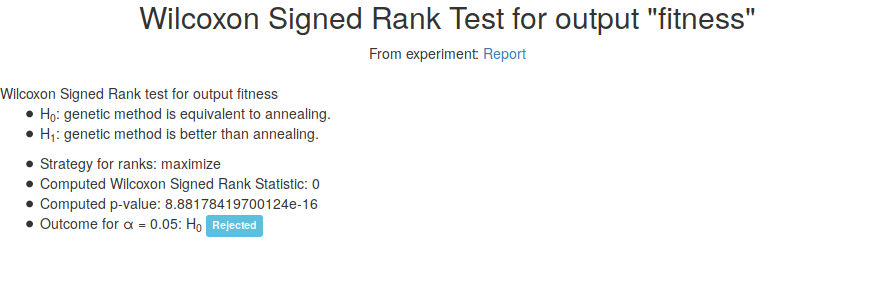
\includegraphics[scale=0.5]{Resultados/bestFitness_output/img/test.png}}
		}
		\caption{GA vs SA: best fitness after 500000 evaluations cap}
		\label{best-fitness}
	\end{figure}
	
	\subsection{Number of evaluations}
	
	Figure \ref{num-evaluations} shows the results of the second type of experiment: comparing GA with SA by checking the number of evaluations of the objective function until finding the optimum value. Note that, in the case that such optimum is not found even with a high evaluation limit, the program will return this maximum value.
	\bigbreak
	As it can be seen on the figures, there is a lot of cases in which one of the algorithms (even the two of them) cannot find the optimum value: in fact, the number of times they get stuck is relatively similar between the two of them, as the Wilcoxon test states: in this sense, both methods are similar.
		
	\begin{figure}
		\subfloat[GA vs SA comparison on number of evaluations until reaching optimum, per-seed]{
			\includegraphics[scale=0.5]{Resultados/numEvaluations_output/img/elem-2.eps}
		}
		\newline
		\subfloat[Wilcoxon paired test result for GA vs SA on number of evaluations for optimum]{
			\fbox{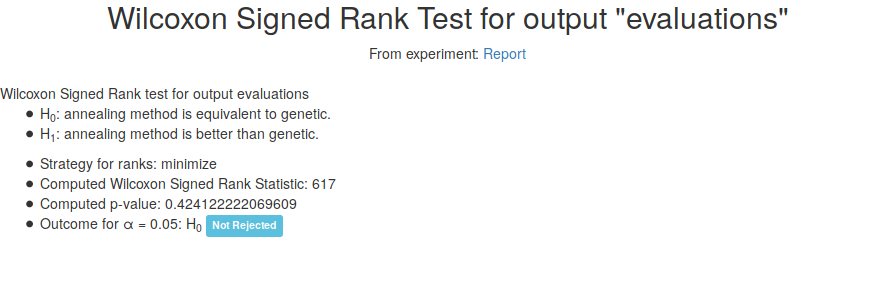
\includegraphics[scale=0.5]{Resultados/numEvaluations_output/img/test.png}}
		}
		\caption{GA vs SA: number of evaluations until reaching optimum}
		\label{num-evaluations}
	\end{figure}
	
	\subsection{Execution time}
	
	Finally, Figure \ref{execution-time} shows the results of the third type of experiment: comparing GA with SA in a way similar to the previous experiment (number of evaluations), but measuring the execution time instead of the number of evaluations.
	\bigbreak
	In this case, as the graphics show, there is a clear dominance of simulated annealing over the genetic algorithm in execution time, except for the cases where SA doesn't find the optimum and GA does. This is further corroborated by the Wilcoxon test, which states that SA is better than GA.
	
	\begin{figure}
		\subfloat[GA vs SA comparison on execution time until reaching optimum, per-seed]{
			\includegraphics[scale=0.5]{Resultados/time_output/img/elem-2.eps}
		}
		\newline
		\subfloat[Wilcoxon paired test result for GA vs SA on execution time for optimum]{
			\fbox{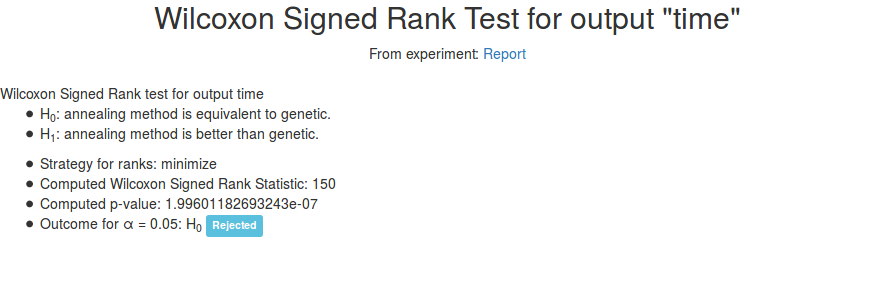
\includegraphics[scale=0.5]{Resultados/time_output/img/test.png}}
		}
		\caption{GA vs SA: execution time until reaching optimum}
		\label{execution-time}
	\end{figure}
	
	\subsection{Results analysis}
	
	By looking at the previous results, the first conclusion that can be drawn is that the genetic algorithm is much better than simulated annealing. This is something that the first statistical test corroborates, with the genetic algorithm outperforming the simulated annealing almost in every experiment instance.
	\bigbreak
	However, there is a catch to this behavior, and	it is that the genetic algorithm is computationally much more expensive than simulated annealing: as it can be seen in Table \ref{alltable} (which represents the numerical values for the results shown in Figure \ref{execution-time}), even the cases in which simulated annealing doesn't find the optimum value in the specified time limit, the time it takes outperforms some cases in which the genetic algorithm finds the optimum!
	\bigbreak
	With this information, it can be concluded that, even if the genetic algorithm is usually better than simulated annealing for finding the optimum, it may not be the best choice in less powerful computers, not only because of its slower speed, but also because of the higher memory consumption: obviously, it is more expensive to keep 256 elements in memory than just 1 or 2. So, there is really no better algorithm: each one will be better suited for some cases. It is also important that, since the statement of the assignment specified so, \underline{these experiments have been run on only one instance of the problem}, so these results may not generalize to other cases.

\begin{table}
\begin{tabular}{ ccc }   % top level tables, with 2 rows
(a) Best fitness & (b) Evaluations & (c) Time \\  
% bottom left of the top level table: table 1 
\begin{tabular}{|l|l|l|}
\hline
    & genetic & annealing \\ \hline
S1  & 10604.0 & 10547.0   \\ \hline
S2  & 10618.0 & 10507.0   \\ \hline
S3  & 10570.0 & 10521.0   \\ \hline
S4  & 10604.0 & 10540.0   \\ \hline
S5  & 10604.0 & 10508.0   \\ \hline
S6  & 10604.0 & 10535.0   \\ \hline
S7  & 10618.0 & 10505.0   \\ \hline
S8  & 10618.0 & 10481.0   \\ \hline
S9  & 10604.0 & 10519.0   \\ \hline
S10 & 10605.0 & 10470.0   \\ \hline
S11 & 10618.0 & 10527.0   \\ \hline
S12 & 10604.0 & 10557.0   \\ \hline
S13 & 10618.0 & 10509.0   \\ \hline
S14 & 10604.0 & 10499.0   \\ \hline
S15 & 10618.0 & 10562.0   \\ \hline
S16 & 10604.0 & 10555.0   \\ \hline
S17 & 10618.0 & 10530.0   \\ \hline
S18 & 10618.0 & 10560.0   \\ \hline
S19 & 10604.0 & 10493.0   \\ \hline
S20 & 10618.0 & 10556.0   \\ \hline
S21 & 10604.0 & 10508.0   \\ \hline
S22 & 10604.0 & 10515.0   \\ \hline
S23 & 10618.0 & 10513.0   \\ \hline
S24 & 10604.0 & 10510.0   \\ \hline
S25 & 10604.0 & 10485.0   \\ \hline
S26 & 10604.0 & 10510.0   \\ \hline
S27 & 10604.0 & 10531.0   \\ \hline
S28 & 10618.0 & 10549.0   \\ \hline
S29 & 10618.0 & 10482.0   \\ \hline
S30 & 10604.0 & 10448.0   \\ \hline
S31 & 10604.0 & 10513.0   \\ \hline
S32 & 10604.0 & 10504.0   \\ \hline
S33 & 10604.0 & 10537.0   \\ \hline
S34 & 10618.0 & 10517.0   \\ \hline
S35 & 10604.0 & 10527.0   \\ \hline
S36 & 10604.0 & 10489.0   \\ \hline
S37 & 10618.0 & 10559.0   \\ \hline
S38 & 10618.0 & 10547.0   \\ \hline
S39 & 10604.0 & 10514.0   \\ \hline
S40 & 10604.0 & 10473.0   \\ \hline
S41 & 10604.0 & 10565.0   \\ \hline
S42 & 10604.0 & 10563.0   \\ \hline
S43 & 10588.0 & 10506.0   \\ \hline
S44 & 10618.0 & 10500.0   \\ \hline
S45 & 10604.0 & 10528.0   \\ \hline
S46 & 10604.0 & 10489.0   \\ \hline
S47 & 10604.0 & 10531.0   \\ \hline
S48 & 10556.0 & 10528.0   \\ \hline
S49 & 10618.0 & 10549.0   \\ \hline
S50 & 10604.0 & 10491.0   \\ \hline
\end{tabular} &
% table 2
\begin{tabular}{|l|l|l|}
\hline
    & genetic & annealing \\ \hline
S1  & 5000256 & 5000001   \\ \hline
S2  & 65934   & 1411988   \\ \hline
S3  & 1833894 & 5000001   \\ \hline
S4  & 5000256 & 1238622   \\ \hline
S5  & 5000256 & 5000001   \\ \hline
S6  & 5000256 & 5000001   \\ \hline
S7  & 51919   & 1265395   \\ \hline
S8  & 55446   & 1450383   \\ \hline
S9  & 5000256 & 5000001   \\ \hline
S10 & 1962343 & 1281357   \\ \hline
S11 & 300473  & 1084357   \\ \hline
S12 & 5000256 & 621064    \\ \hline
S13 & 90466   & 1040709   \\ \hline
S14 & 5000256 & 5000001   \\ \hline
S15 & 38949   & 5000001   \\ \hline
S16 & 5000256 & 1381314   \\ \hline
S17 & 175649  & 5000001   \\ \hline
S18 & 36047   & 1175571   \\ \hline
S19 & 5000256 & 5000001   \\ \hline
S20 & 54638   & 5000001   \\ \hline
S21 & 5000256 & 5000001   \\ \hline
S22 & 5000256 & 5000001   \\ \hline
S23 & 32888   & 1509057   \\ \hline
S24 & 5000256 & 5000001   \\ \hline
S25 & 5000256 & 1631830   \\ \hline
S26 & 5000256 & 5000001   \\ \hline
S27 & 5000256 & 5000001   \\ \hline
S28 & 11626   & 5000001   \\ \hline
S29 & 43104   & 5000001   \\ \hline
S30 & 5000256 & 5000001   \\ \hline
S31 & 5000256 & 5000001   \\ \hline
S32 & 5000256 & 1442029   \\ \hline
S33 & 5000256 & 5000001   \\ \hline
S34 & 45974   & 5000001   \\ \hline
S35 & 5000256 & 861258    \\ \hline
S36 & 5000256 & 5000001   \\ \hline
S37 & 44920   & 5000001   \\ \hline
S38 & 61710   & 940714    \\ \hline
S39 & 5000256 & 1250205   \\ \hline
S40 & 5000256 & 1438560   \\ \hline
S41 & 5000256 & 1146254   \\ \hline
S42 & 5000256 & 1472901   \\ \hline
S43 & 5000256 & 1510448   \\ \hline
S44 & 52011   & 1399984   \\ \hline
S45 & 5000256 & 1322201   \\ \hline
S46 & 5000256 & 5000001   \\ \hline
S47 & 5000256 & 5000001   \\ \hline
S48 & 5000256 & 1358309   \\ \hline
S49 & 111050  & 5000001   \\ \hline
S50 & 5000256 & 5000001   \\ \hline
\end{tabular} &
% asdf
\begin{tabular}{|l|l|l|}
\hline
    & genetic & annealing \\ \hline
S1  & 10341   & 1556      \\ \hline
S2  & 154     & 478       \\ \hline
S3  & 3918    & 1625      \\ \hline
S4  & 10608   & 446       \\ \hline
S5  & 11202   & 1595      \\ \hline
S6  & 11070   & 1539      \\ \hline
S7  & 143     & 447       \\ \hline
S8  & 142     & 535       \\ \hline
S9  & 11369   & 1637      \\ \hline
S10 & 4193    & 458       \\ \hline
S11 & 668     & 370       \\ \hline
S12 & 10270   & 229       \\ \hline
S13 & 197     & 372       \\ \hline
S14 & 10315   & 1607      \\ \hline
S15 & 115     & 1618      \\ \hline
S16 & 10720   & 511       \\ \hline
S17 & 373     & 1631      \\ \hline
S18 & 113     & 417       \\ \hline
S19 & 10993   & 1540      \\ \hline
S20 & 136     & 1553      \\ \hline
S21 & 10677   & 1523      \\ \hline
S22 & 10629   & 1600      \\ \hline
S23 & 101     & 520       \\ \hline
S24 & 10920   & 1584      \\ \hline
S25 & 10733   & 554       \\ \hline
S26 & 10685   & 1475      \\ \hline
S27 & 9198    & 1568      \\ \hline
S28 & 59      & 1599      \\ \hline
S29 & 107     & 1563      \\ \hline
S30 & 10370   & 1396      \\ \hline
S31 & 10913   & 1600      \\ \hline
S32 & 10357   & 498       \\ \hline
S33 & 10296   & 1469      \\ \hline
S34 & 108     & 1531      \\ \hline
S35 & 10397   & 309       \\ \hline
S36 & 10341   & 1589      \\ \hline
S37 & 111     & 1550      \\ \hline
S38 & 161     & 350       \\ \hline
S39 & 10682   & 429       \\ \hline
S40 & 10472   & 477       \\ \hline
S41 & 10150   & 391       \\ \hline
S42 & 10628   & 520       \\ \hline
S43 & 11528   & 519       \\ \hline
S44 & 139     & 494       \\ \hline
S45 & 10882   & 463       \\ \hline
S46 & 10902   & 1622      \\ \hline
S47 & 10585   & 1507      \\ \hline
S48 & 10924   & 451       \\ \hline
S49 & 221     & 1526      \\ \hline
S50 & 10417   & 1522      \\ \hline
\end{tabular} \\
\end{tabular}
\caption{Detailed results for the experiments performed. Note that S1 refers to seed value 0, S2 refers to seed value 1, and so on. Also, the results on b) and c) have been drawn from the same execution.}
\label{alltable}
\end{table}
	
	\section{Conclusions} \label{Conclusions}
	
	In this assignment, a comparison between a genetic algorithm and simulated annealing has been performed over a specific instance of the knapsack problem. In order to do so, a code has been downloaded and modified in order to include both the knapsack problem and the SA algorithm, in addition to some more modifications to ease the process of collecting results. Then, experiments have been run and processed through a tool to extract statistical information. From these results, it has been concluded that, while GA usually outperforms SA in finding the optimum, SA uses much less computational resources, so each one is well-suited for different scenarios.
	
	\begin{thebibliography}{9}
		\bibitem{codigoga} Enrique Alba, \textit{ssGA: Steady State GA}. \texttt{http://neo.lcc.uma.es/software/ssga/index.php}
		\bibitem{knapsack} J. E. Beasley, \textit{Multidimensional knapsack problem}. \texttt{http://people.brunel.ac.uk/\~ \ mastjjb/jeb/orlib/mknapinfo.html}
		\bibitem{saparam} Juan Frausto-Solis, E.F. Roman, David Romero, Xavier Soberon, and Ernesto Liñan-Garcia, \textit{Analytically Tuned Simulated Annealing Applied to the Protein Folding Problem}. In Computational Science-ICCS 2007 (pp. 370-377)
		\bibitem{exreport} J. Arias, J. Cozar, \textit{exreport: An R package for easy reproducible research}. \texttt{http://exreport.jarias.es/}
	\end{thebibliography}
	
\end{document}
